
\section{Approach}
%
%Describe the final approach you are take for this problem.
%For instance, here you would describe the details of the network’s
%architecture. What training parameters and techniques you have used.
%The computational complexity of your model. And similar questions.
%To help explain your approach please make figures to accompany your
%text description. (1-3 pages)
For our research we replicated the DCGAN network, described in great detail in \cite{DBLP:journals/corr/RadfordMC15}, in Tensorflow using Taehoon Kim's (found \href{https://github.com/carpedm20/DCGAN-tensorflow}{here}) implementation as inspiration.
\subsection{Network Architecture}
\paragraph{Generator architecture details.} The generator's input layer is a vector of size 100 followed by 4 convolutional hidden layers. The output layer is then the picture generated that feeds into the discriminator. The 4 hidden layers use the ReLU activation function(Eq.(\ref{relu-equation})) while the output layer uses the $\tanh$ function(Eq.(\ref{tanh-equation})). The authors of DCGAN state that using a bounded activation like $\tanh$ for the output layer allowed the network to \textit{"learn more quickly to saturate and cover the color space of the training distribution"}(p. 3).
\paragraph{Discriminator architecture details}. The discriminator's architecture  follows a very similar structure with the obvious exception of the input and output layers. The input layer for the discriminator consists of an image, while the output layer is a single neuron activated by a $sigmoid$ function that represents the classification of real vs fake images. The convolutional layers use the leaky relu function (Eq.(\ref{lrelu-equation})). \\
Both networks were trained using the Adam optimizer \cite{2014arXiv1412.6980K} with a learning rate of 0.002, as advised by the authors of DCGAN.

%Within the
%discriminator we found the leaky rectified activation (Maas et al., 2013) (Xu et al., 2015) to work
%well, especially for higher resolution modeling. This is in contrast to the original GAN paper, which
%used the maxout activation (Goodfellow et al., 2013).
\begin{equation}
\label{relu-equation}
x = max(0, x)\\
\end{equation}

\begin{equation}
\label{tanh-equation}
\tanh x = \frac{1 - e^{-2x}}{1 + e^{-2x}}
\end{equation}

\begin{equation}
\label{lrelu-equation}
       lrelu = 
        \begin{cases}
            x & \text{if $x > 0$} \\
            0.01x & \text{otherwise}
        \end{cases}
\end{equation}


\begin{figure}[h]
\centering
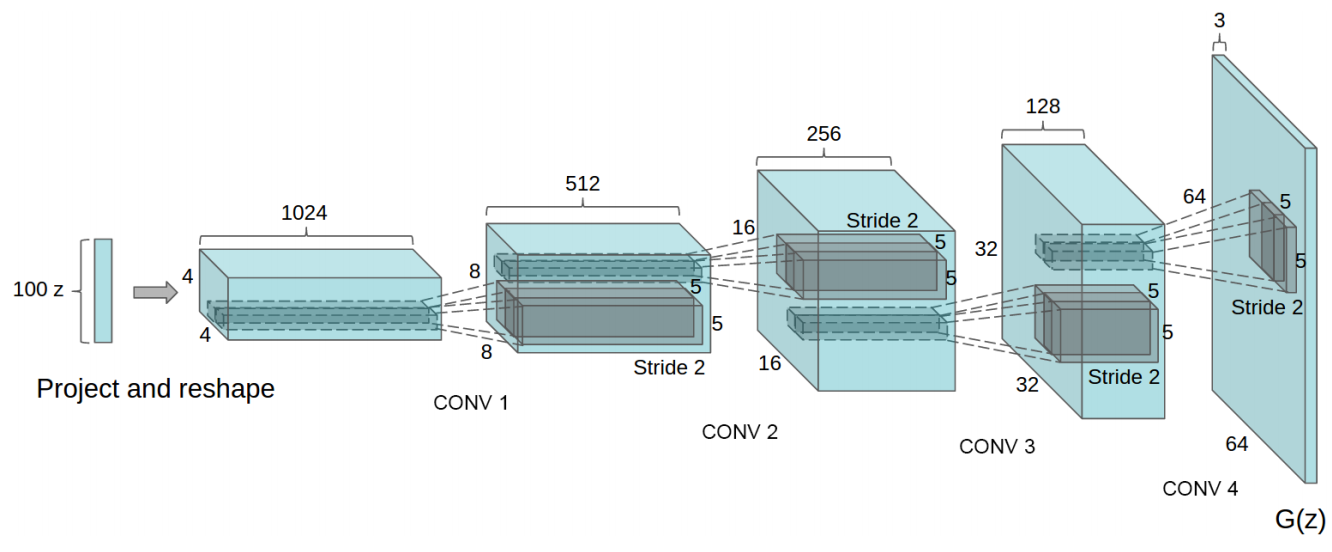
\includegraphics[width=\textwidth]{figures/DCGAN.png}
\caption{Generator Network architecture. Cited from \cite{DBLP:journals/corr/RadfordMC15} }
\label{fig:architecture}
\end{figure}

\subsection{Network Training}
Due to the complexity of the networks we did all of our experiments on two separate GPU enabled devices. We ran most of our experiments on a laptop that has a NVIDIA GTX 1060 GPU while some training iterations were done using a Amazon Web Service EC2 Deep Learning instance with a NVIDIA K80 GPU. Even though utilizing these machines made our training much faster, each training iteration took a considerable amount of time. This resulted in us having to run our experiments over night and use the days to implement our networks and interpret the results. 

\subsection{Data Collection}
%not sure if this is actually something we want to include and if so where it should be introduced so feel free to change it
%TODO possibly add a reference instead of the hyperlink

During experimentation we mostly relied on the popular benchmark dataset \href{https://www.cs.toronto.edu/~kriz/cifar.html}{CIFAR10}, however an additional data set was collected using \href{https://www.flickr.com/services/api/}{Flickr's API}. Due to varying amounts of quality pictures of objects that would be interesting to base the image generation on, a collection that included mostly different reptiles with a fair amount of arachnid's thrown into the mix was ultimately settled upon, this data set will be referred to as the Reptiles data set from here on. In total the data set is made up of approximately 20K color images all re-sized to dimensions of 108x108x3 before training was conducted. Examples of images can be seen in figure \ref{fig:reptiles}.


\begin{figure}[H]
\centering
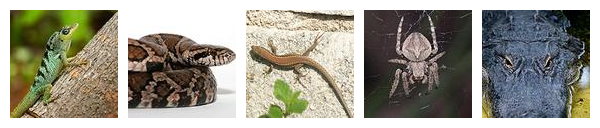
\includegraphics[width=\textwidth]{figures/reptiles.png}
\caption{Examples from the Reptiles data set}
\label{fig:reptiles}
\end{figure}
